%!TEX root = project_description.tex

%%%%%%%%%%%%%%%%%%%%%%%%%%%%%%%%%
\section{Timeline and Milestones}
\label{sec:timeline}
%%%%%%%%%%%%%%%%%%%%%%%%%%%%%%%%%

The timeline for this project is organized by three major tasks labeled Thrust \#1, Thrust \#2, and Thrust \#3, and also includes a timeline for broader impact activities.
Thrust \#1 involves completing our preliminary investigation into the use of FRP in both deterministic and stochastic CRNs.
During this time, we will finish our Haskell implementation of FRP constructs for CRNs, evaluate their strengths and weaknesses, and begin a deeper investigation into an FRP language for stochastic CRNs, employing signal functions over arbitrary probability distributions.
Thrust \#2 develops new domain specific languages for specifying deterministic and stochastic CRNs in a functional reactive programming style.
The features and type system of these languages will be informed from our preliminary results from Thrust \#1 and integrate temporal logic elements inspired by LTL.
Thrust \#3 includes a meta-theoretic analysis of these languages and the development of supportive software tools.
All of the thrusts, included the broader impact activities will be carried out simultaneously over the four years.
Theses thrusts are further divided into several tasks, and appear in the time line chart below.
A lead investigator(s) is also indicated for each task determined by the expertise of the investigator in the specific task.

\begin{figure}[h!]
     \centering
     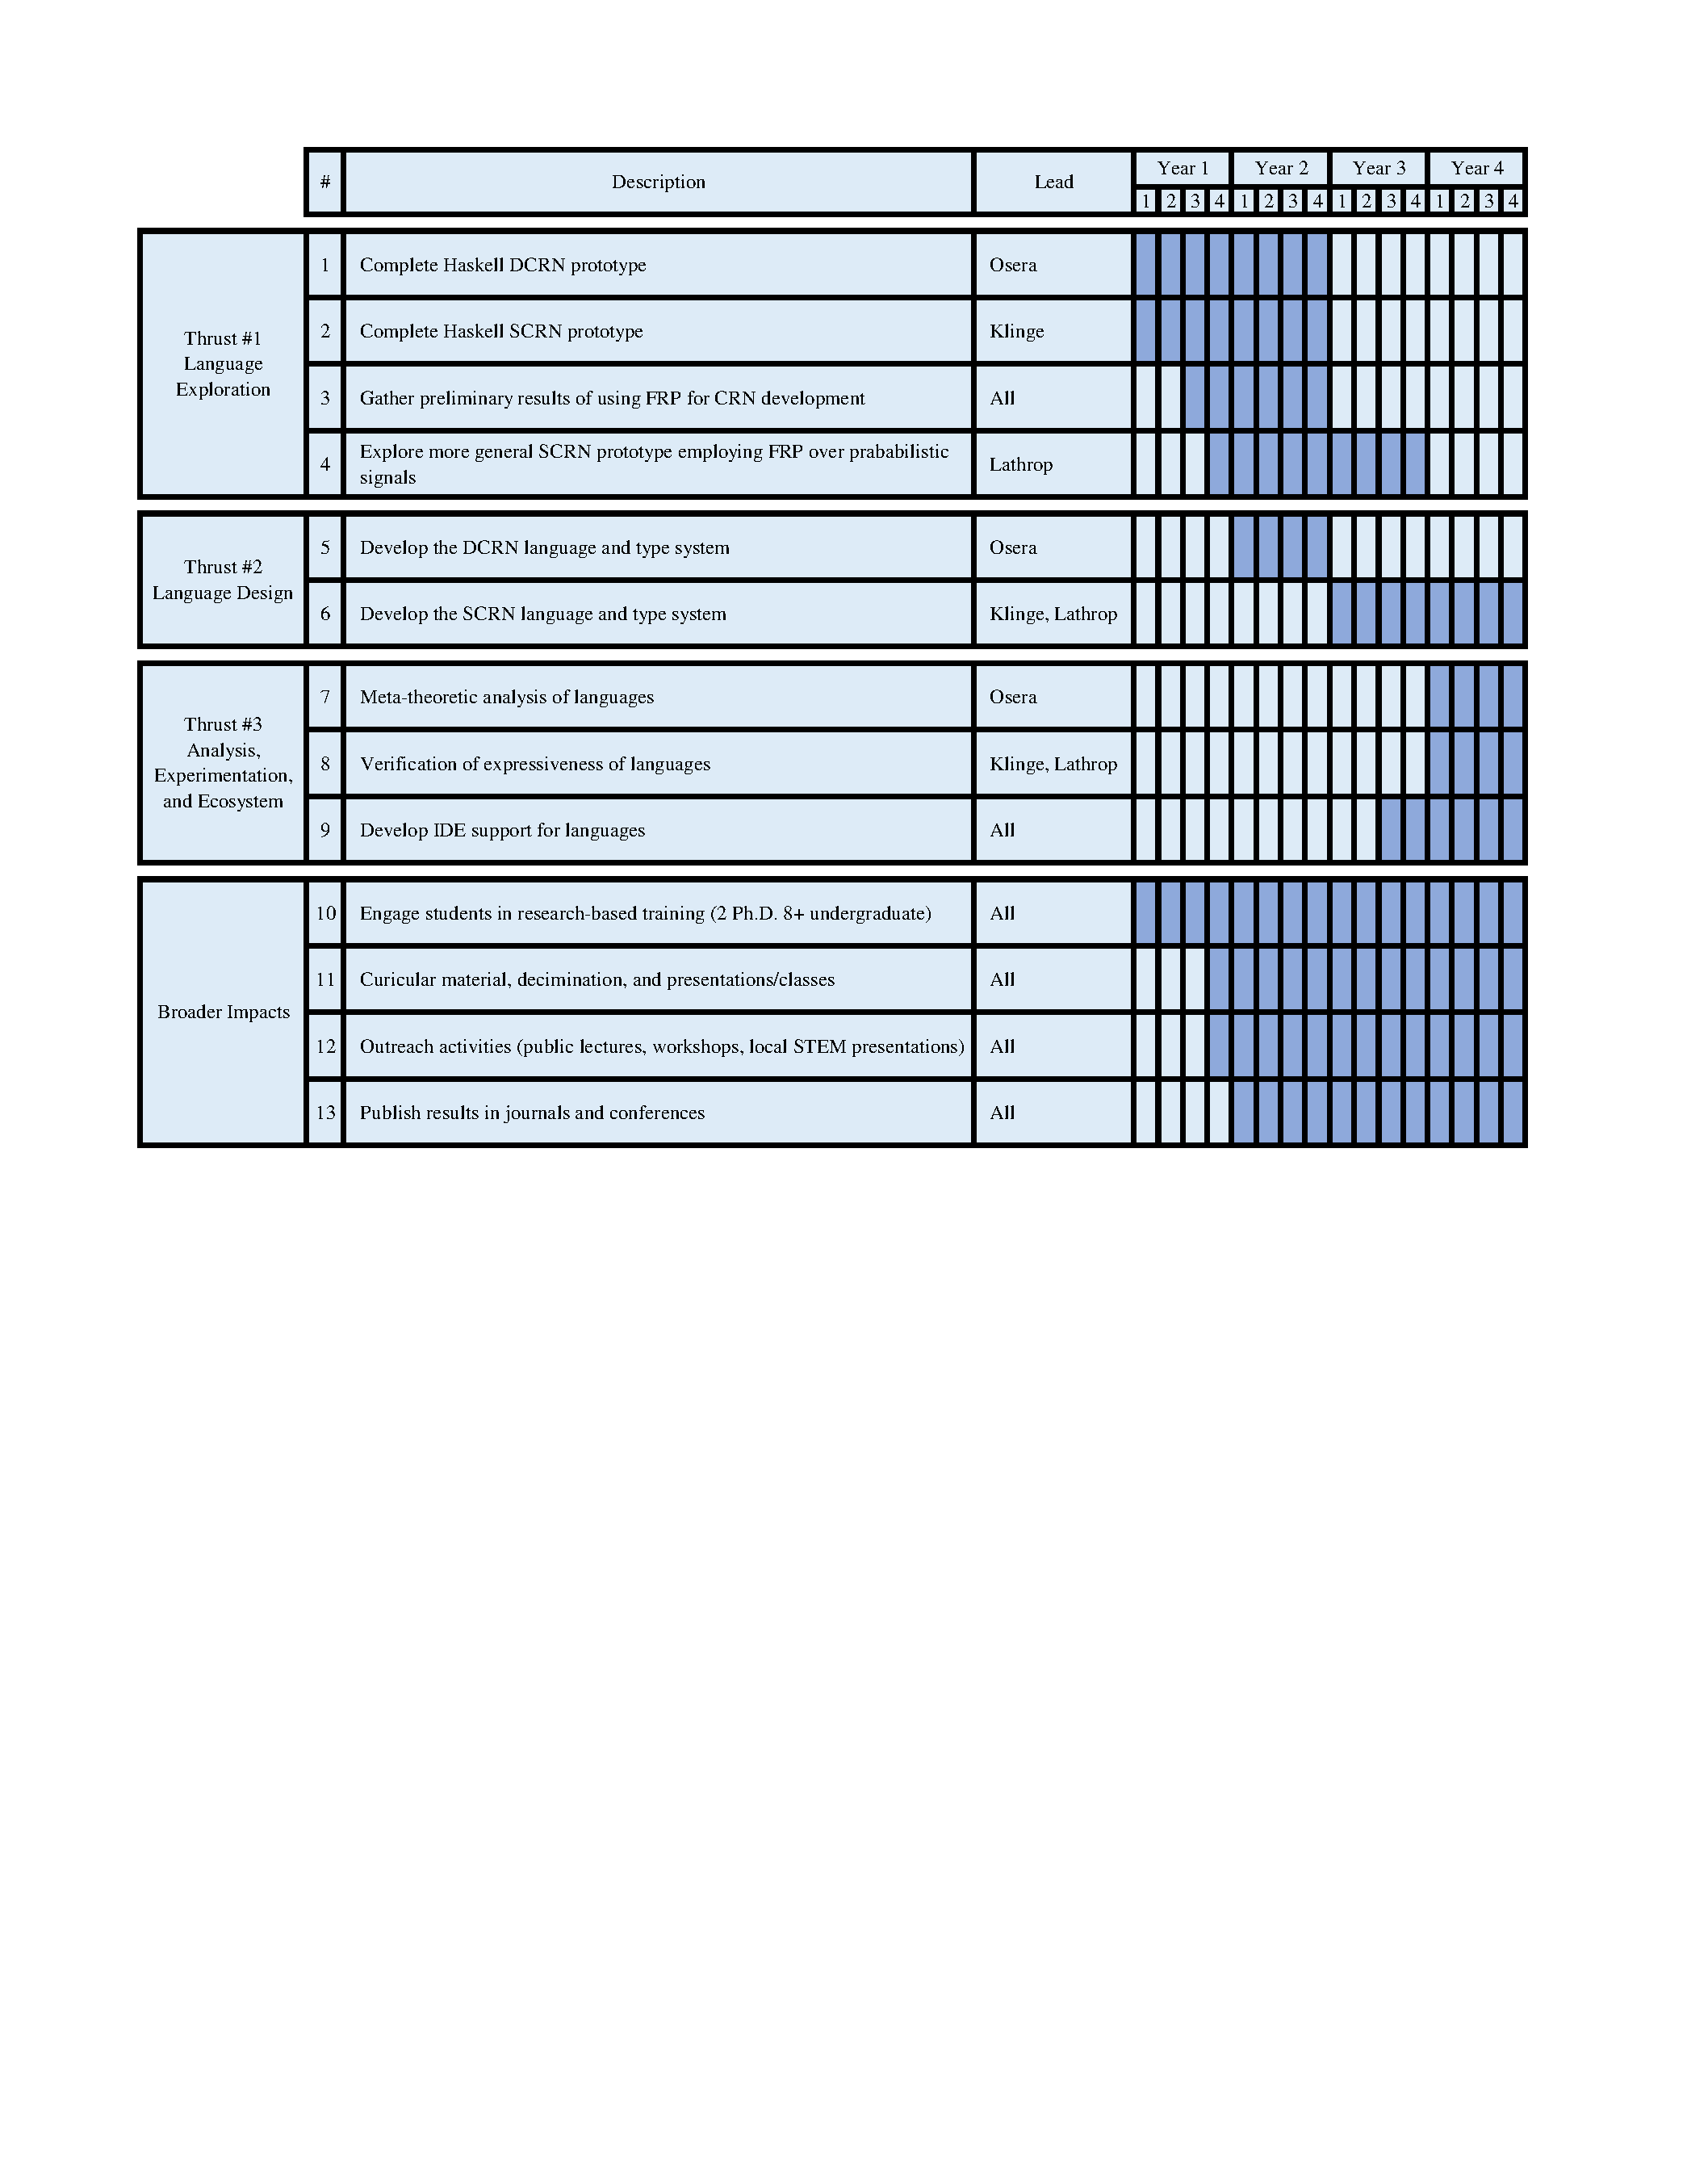
\includegraphics[width=6.4in]{TimeLine.pdf}
     \caption{Project Timeline}
 \end{figure}


